\section{Task 3: Climax Technology's Vesta platform} \label{ch:pentesting:vesta}
Climax Technology, the manufacturer of the hardware used in this system, does not seem to be a consumer-facing business. Nonetheless, they have their own software platform to control their system, called \textit{Vesta}. In the SecuritasHome system, this platform and its components are essentially replaced by \textit{Alarm.com}. The Vesta platform features a mobile application\footnotelink{https://play.google.com/store/apps/details?id=com.climax.vestasmarthome.eu}{2021-04-20} to control the system, as well as a web portal\footnotelink{https://eu.vestasmarthome.com/Vesta/}{2021-04-20}. A potential security vulnerability is if this Vesta platform is still active and usable to control this system.

\subsection{Background}
As stated above, Climax Technology have their own platform, branded as Vesta, to control the system. A common vulnerability in IoT devices is not covering up vulnerabilities arising higher up in the supply chain (\todo source). In this system, there is a possibility that \textit{Alarm.com} has not properly deactivated the access and functionality of the Vesta platform. The idea is for the Alarm.com platform to replace it entirely.

In the app \textit{Vesta Home 5 EU}, see figure \ref{fig:vesta-home-app}, one can perform essentially all actions that the Alarm.com mobile application provides (see section \ref{ch:system:software}). On the landing page, you are greeted with simple a login page (where your Alarm.com credentials don't work). However, it also includes a button labeled \textit{First Time Registration} (see figure \ref{fig:vesta-landing-page}), where one can register a new account connected to a new system. To register a new system one only needs to enter its MAC address, see \ref{fig:vesta-registration-page}, which is available without authorization from the local admin page (see \ref{ch:system:software}). Potentially, one could then register the system in the Vesta platform to gain authorization to control the system, thus bypassing the security completely.
\begin{figure}[!ht]
    \centering
    \begin{subfigure}[t]{0.4\textwidth}
        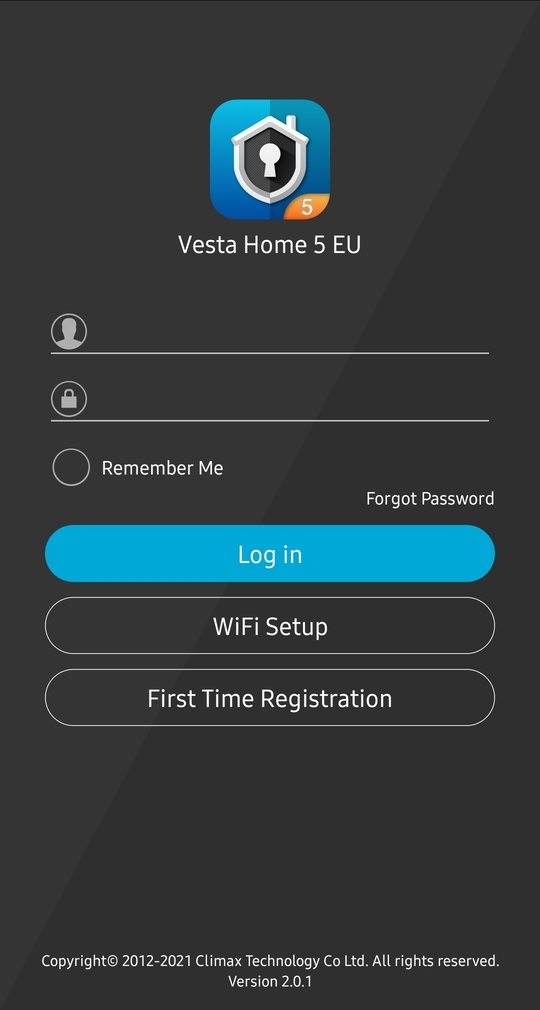
\includegraphics[height=3.8in]{images/6-pentesting/vesta-home-landing-page.jpg}
        \caption{The landing page}
        \label{fig:vesta-landing-page}
    \end{subfigure}%
    ~
    \begin{subfigure}[t]{0.4\textwidth}
        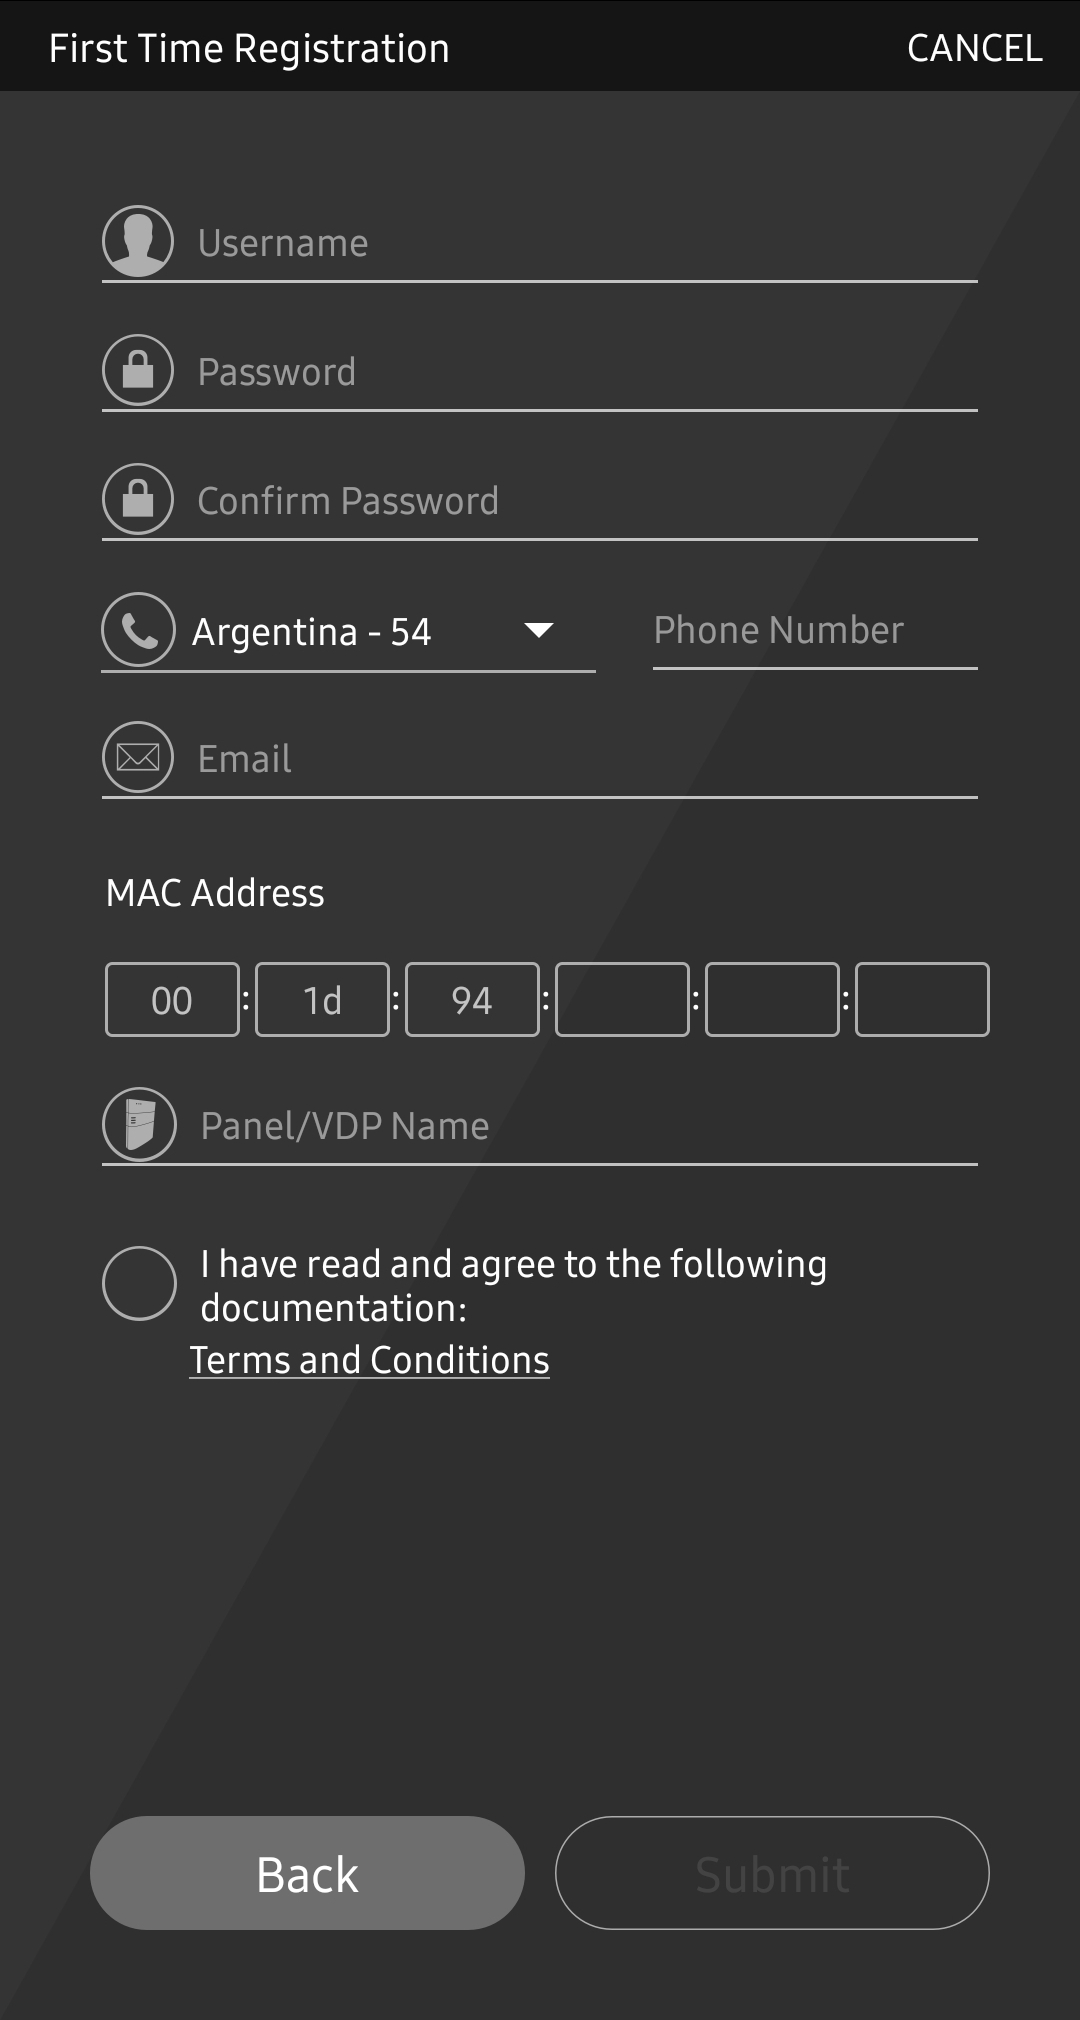
\includegraphics[height=3.8in]{images/6-pentesting/vesta-home-registration.jpg}
        \caption{The "First Time Registration" page}
        \label{fig:vesta-registration-page}
    \end{subfigure}
    \caption{The Vesta Home 5 EU mobile application.}
    \label{fig:vesta-home-app}
\end{figure}
In the Vesta web application, there is a very similar form, allowing you to register a new device using the MAC address, see figure \ref{fig:vesta-web-registration}.
\begin{figure}[!ht]
    \centering
    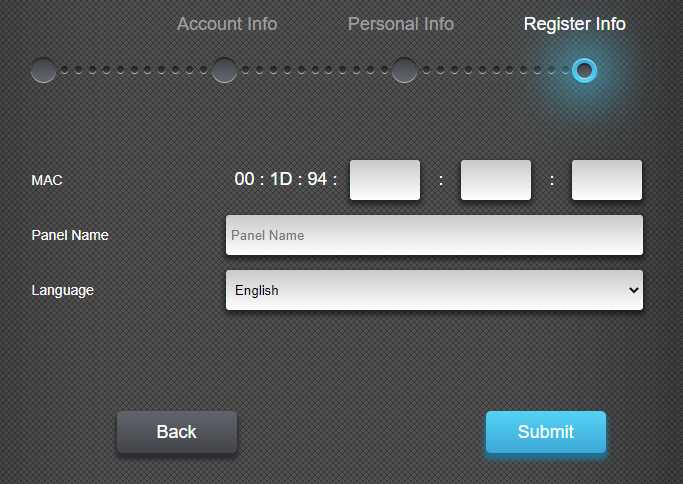
\includegraphics[width=0.9\textwidth]{images/6-pentesting/vesta-web-registration.png}
    \caption{The Vesta web application registration.}
    \label{fig:vesta-web-registration}
\end{figure}

\subsection{Method}
The mobile application is free to download. To be able to confidently monitor the network traffic, the mobile application was installed on an android emulator for PC, and Wireshark was run on the host machine.

Both applications use HTTPS, meaning the requests are encrypted. An attempt was made to perform a \gls{MITM} attack on the mobile application to view the HTTPS traffic, using \textit{mitmproxy}\footnotelink{https://mitmproxy.org/}{2021-04-21} and the built-in proxy settings of the android emulator. However, this made the application yield an error message saying it could not reach the server. Presumably, the application uses certification pinning to protect against this type of attack. This was not explored further since the traffic can easily be viewed in the web application, using the Chrome network tab (see figure \ref{fig:vesta-web-registration-failed}), and most likely both applications access the same API.

\subsection{Results}
The penetration test was unsuccessful. Both the mobile application and the web application yielded identical results. A simple error message is shown, saying the \textit{MAC/IMEI} is incorrect, see figures \ref{fig:vesta-home-registration-failed} and \ref{fig:vesta-web-registration-failed}. In the Chrome network tab, we can see when trying to register the system through the web application that the API responds with the message "no data found!".
\begin{figure}[!ht]
    \centering
    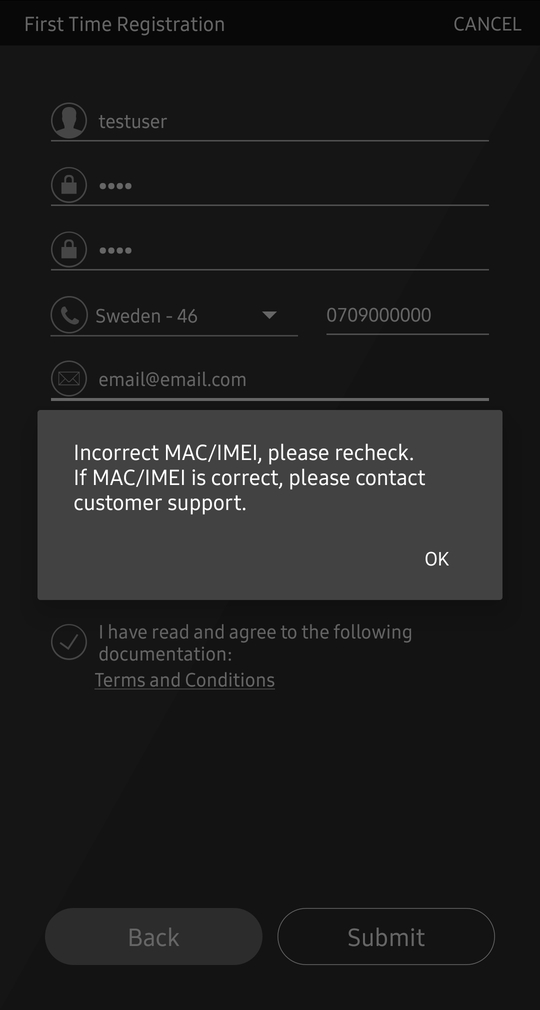
\includegraphics[width=0.4\textwidth]{images/6-pentesting/vesta-home-registration-failed.jpg}
    \caption{The results of trying to register in the Vesta mobile app.}
    \label{fig:vesta-home-registration-failed}
\end{figure}
\begin{figure}[!ht]
    \centering
    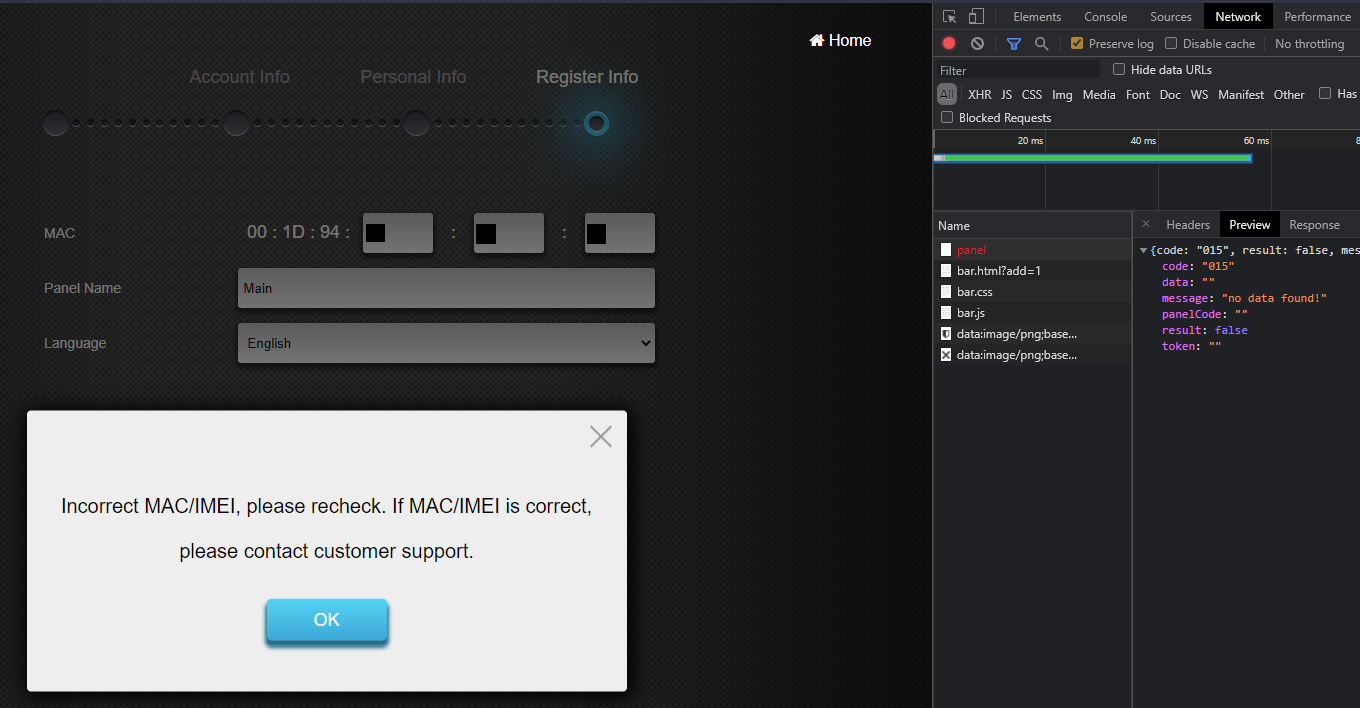
\includegraphics[width=0.9\textwidth]{images/6-pentesting/vesta-web-registration-failed.png}
    \caption{The results of trying to register in the Vesta web app.}
    \label{fig:vesta-web-registration-failed}
\end{figure}

\subsection{Discussion}
Trying to register the hardware to the Vesta platform was unsuccessful. The given MAC address was not accepted. Presumably, Climax Technology has a database of the MAC addresses of all sold systems under the Vesta platform. While the MAC address of the system in this thesis is registered under Climax Technology, it does not seem to be registered by the Vesta platform. Another possibility is that the MAC address and IMEI number pair is not registered because \textit{Alarm.com} has used their own SIM cards and thus a different IMEI number. This is indicated by the error messages shown. Which of these scenarios is the correct one, we cannot know. Either way, we can see that the API responds with a negative result, saying that no data could be found. Therefore, this type of supply chain error seems to have been identified and correctly protected against.
